% Atlas Workbench scoring white paper — LaTeX edition of WHITEPAPER_v2.md
% (paper revision 2, 2026-08-03). Content is the amended edition produced in
% response to WHITEPAPER_REVIEW.md; the Markdown file remains the canonical
% content + audit-trail lineage. Template follows tslit-dspy whitepaper
% conventions.
\documentclass[11pt]{article}
\usepackage[margin=1in]{geometry}
\usepackage{amsmath,amssymb}
\usepackage{graphicx}
\graphicspath{{../figures/}{./figures/}}
\usepackage{booktabs}
\usepackage{hyperref}
\usepackage{titlesec}
\usepackage{enumitem}
\usepackage{xcolor}
\usepackage{tcolorbox}
\tcbuselibrary{skins}
\usepackage{mdframed}
\usepackage[protrusion=true,expansion=false]{microtype}
\usepackage{parskip}
% many \texttt{identifiers} in prose: allow extra stretch instead of overfull lines
\setlength{\emergencystretch}{1.5em}
% bibliography uses manual \bibitem with hardcoded author-year text

\definecolor{darkblue}{HTML}{1A3A5C}
\definecolor{darkred}{HTML}{8B1A1A}
\definecolor{midred}{HTML}{C0392B}
\definecolor{midblue}{HTML}{2C5F8A}
\definecolor{lightblue}{HTML}{D6E8F7}
\definecolor{darkgreen}{HTML}{1A6B3C}
\definecolor{warnorange}{HTML}{E67E22}

\titleformat{\section}{\large\bfseries\color{darkblue}}{\thesection}{0.6em}{}
\titleformat{\subsection}{\normalsize\bfseries\color{darkblue}}{\thesubsection}{0.6em}{}
\titleformat{\subsubsection}{\normalsize\bfseries\color{midblue}}{\thesubsubsection}{0.6em}{}

\hypersetup{
  colorlinks=true,
  linkcolor=darkblue,
  urlcolor=midblue,
  citecolor=darkblue
}

\tcbset{
  boxrule=0.8pt,
  colback=lightblue!30,
  colframe=darkblue,
  fonttitle=\bfseries\small,
  attach boxed title to top left={yshift=-2mm,xshift=4mm},
  left=6pt, right=6pt, top=4pt, bottom=4pt
}

% -----------------------------------------------------------------------
\title{%
  \vspace{-0.5cm}%
  {\color{darkblue}\LARGE\bfseries Rating Compound Operational-Risk Scenarios}\\[6pt]
  {\color{darkred}\Large\bfseries A Deterministic Scoring Algorithm\\ with Pre-Registered Falsification}\\[10pt]
  {\large\normalfont Atlas Workbench white paper --- scoring engine\\
   (\texttt{algorithm\_version} 0.1.0)}
}
\author{%
  Nicolas Cravino\\
  \small\textit{Paper revision 2 --- August 3, 2026}\\[6pt]
  \small\textit{Amended after an adversarial full-repo review; v1 preserved as the reviewed artifact}
}
\date{}

% -----------------------------------------------------------------------
\begin{document}
\maketitle

\begin{tcolorbox}[title=Key Findings --- stated the way a validator would state them]
On the pre-registered synthetic regime the dependence-aware scorer beats the
independence baseline by \textbf{84\% relative average precision} --- a bar
\S\ref{sec:taskb} shows the synthetic generator made structurally easy ---
and beats the strong shared-channel baseline, \emph{which on this regime is
an oracle holding the planted answer key}, by \textbf{+5.2\% AP} and
\textbf{0.90-vs-0.80 precision-at-20}, while losing to it on AUROC. A
harness utility recovers planted dependence structure at \textbf{77\%
precision} against a 29\% random floor (48\% among co-occurring pairs).

The same harness documents what fails: atom-frequency calibration loses to a
pooled baseline on the decision regime, the public-regime task fails on
sparsity --- \textbf{so the dependence layer has yet to influence a single
production number} --- and the shipped estimator prices rare,
never-co-observed pairs \emph{below} independence, a defect the ranking-only
evaluation cannot see (\S\ref{sec:defects}).
\end{tcolorbox}

\begin{tcolorbox}[title=Disclaimer, colframe=darkred, colback=red!4]
Outputs are hypothetical research artifacts. Scenario scores express model
assumptions and prioritization choices, not calibrated probabilities or
forecasts. They are not financial, legal, regulatory, investment, security,
or risk-management advice, and they are not capital parameters. See
\texttt{DISCLAIMER.md} in the repository root.
\end{tcolorbox}

\begin{center}\small
\begin{tabular}{@{}lp{0.78\linewidth}@{}}
\toprule
Status & Implemented and evaluated on the synthetic R0 regime; research-tier per the model inventory \\
Revision & 2 --- amended per \texttt{WHITEPAPER\_REVIEW.md}; change map in \texttt{WHITEPAPER\_v2\_REVISION\_LOG.md} \\
Companion & \texttt{HYBRID\_SCORING\_PROPOSAL.md} (scheduled algorithm fixes and judgment-channel design) \\
Specification & \texttt{docs/research/redesignv1/algorithm-spec.md} \\
Implementation & \texttt{workbench\_atlas/scoring/} \\
Evaluation & \texttt{generated/redesign/} --- reproducible via Appendix~\ref{app:repro}; not under version control (Appendix~\ref{app:evidence}) \\
\bottomrule
\end{tabular}
\end{center}

\section*{Executive Summary (plain language)}

\emph{This section is for readers who are not statisticians. It says what
the system does, what the unavoidable jargon means, and what the results do
and do not show --- at the same level of honesty as the technical sections,
just without the mathematics. A glossary follows it.}

Institutions prepare for risks one at a time; the events that actually hurt
are usually \textbf{combinations} --- a control failure, a concentrated
supplier, and an external shock landing in the same quarter. This system
finds and scores those combinations, and it does so with a method
deliberately built from components a bank's model-validation team already
knows how to challenge.

\textbf{The approach, in plain terms.} Each single risk from the register
is treated as an indivisible building block --- a \textbf{risk atom}. The
``decomposition per risk atom'' means each block is split into two
separately estimated questions: \emph{how often does this happen?} and
\emph{how bad is it when it does?} The system then asks the data how often
two blocks have actually struck \textbf{together}, starting from a
skeptic's assumption --- no connection --- and moving away from it only as
evidence accumulates. Because the arithmetic of rare combinations has no
clean formula, the final step is a \textbf{Monte Carlo} simulation:
rehearse the coming year twenty thousand times, count how often the
combination lands, and record what it costs when it does. (Monte Carlo is
nothing more mysterious than dice-rolling at industrial scale --- the same
family of simulation used for modeling attack paths in security
engineering; for a practitioner-level treatment of simulation-driven
defense see the author's book~\cite{cravino_book}.) A final overlay borrows
from \textbf{extreme-value theory} --- the statistics of worst cases --- to
give a second opinion on the most severe outcomes, and that overlay must
pass its own stability test or it is thrown away.

What is actually new here is not the mathematics --- every component is
deliberately standard. The innovation is \textbf{discipline}: the pass
marks for every test were written down \emph{before} the tests were run;
the failures are published next to the passes; every published number can
be reconstructed from stored files; and no AI language model writes or
influences any number --- models draft prose for humans, never scores.

\textbf{What the results honestly say.} On a simulated world where the true
answer was planted, the system recovers the planted structure and modestly
out-ranks a reference method that was effectively handed the answer key ---
strong evidence the machinery works, not yet evidence about the real world.
On real public data there is not yet enough shared history for the
dependence layer to add anything: today its production output matches the
naive method, and this paper says so. One known flaw is disclosed rather
than hidden: the current estimator \emph{under}-prices exactly the rarest
never-yet-seen combinations --- the very thing the product exists to
surface --- and the designed fix will be adopted only if it wins a
pre-registered test. Loss-size estimates are not yet validated at all.
Until that changes, every output is a \textbf{research quantity}: useful
for prioritization and challenge, not a probability to act on, and never a
capital or business input.

\subsection*{Plain-language key to the jargon}

\begin{center}\footnotesize
\begin{tabular}{@{}p{0.25\linewidth}p{0.70\linewidth}@{}}
\toprule
Term & What it means here \\
\midrule
Risk atom & One single risk from the register, treated as an indivisible
building block (e.g.\ ``identity-provider outage''). \\
Compound scenario & Two or more atoms striking in the same window --- the
thing this paper rates. \\
Decomposition per risk atom & Splitting each risk into ``how often?''
(frequency) and ``how bad?'' (severity), estimated separately and then
recombined. \\
Dependence / co-occurrence & The tendency of risks to strike together
because they share plumbing (same cloud provider, same funding model, same
regulator). Measured by counting quarters in which both actually fired. \\
Shrinkage prior & The skeptic's starting point: assume no connection until
the data argues otherwise. Thin evidence moves the estimate a little;
strong evidence moves it a lot. \\
Monte Carlo & Rehearsing the coming year many thousands of times in
simulation and counting the outcomes, because rare-combination arithmetic
has no clean closed formula. Named after the casino. \\
Tail / extreme-value theory (EVT) & The worst few percent of outcomes, and
the branch of statistics built to estimate them. Used here as a second
opinion that must pass a stability check or be discarded. \\
Pre-registration & The pass marks were written down before the tests were
run, so results cannot quietly move the goalposts. Failures are published
beside passes. \\
Holdout & Data kept locked away while the model is fitted and used only
for the final exam. \\
Calibration & Whether stated probabilities match reality: when the system
says ``10\%'', does it happen about one time in ten? \\
Audit blob / realization & The stored file from which every published
digit can be reconstructed, down to the random seed. \\
Research quantity & A number for prioritization and challenge --- not a
validated probability, and never a capital or business input. \\
\bottomrule
\end{tabular}
\end{center}

\newpage

\begin{abstract}
Banks are not surprised by single risks; they are surprised by
\emph{combinations} --- a control failure, a third-party concentration, and
an external shock that materialize together. Atlas Workbench rates such
\textbf{compound scenarios} with a deliberately conservative algorithm:
standard frequency $\times$ severity decomposition per risk atom, a
shrunk-empirical dependence estimator, Monte Carlo propagation under an
explicit occurrence definition, and a peaks-over-threshold EVT tail overlay
with a built-in falsification rule. Every evaluation-path score persists its
full component decomposition so a validator can reconstruct it --- exactly,
up to the hash-coverage gaps \S\ref{sec:versioning} itemizes; the production
path does not yet honor even that much, and \S\ref{sec:gaps} says so. The
algorithm is deterministic end to end: no large language model (LLM)
participates in scoring. On the pre-registered synthetic regime, the
dependence-aware scorer beats the independence baseline by 84\% relative
average precision --- a bar \S\ref{sec:taskb} shows the synthetic generator
made structurally easy --- and beats the strong shared-channel baseline,
which on this regime is an oracle holding the planted answer key, by 5.2\%
AP and 0.90-vs-0.80 precision-at-20, while losing to it on AUROC. A harness
utility recovers planted dependence structure at 77\% precision against a
29\% random floor (48\% among co-occurring pairs). The same harness
documents what fails: atom-frequency calibration loses to a pooled baseline
on the decision regime, the public-regime task fails on sparsity --- so the
dependence layer has yet to influence a single production number --- and the
shipped estimator prices rare, never-co-observed pairs \emph{below}
independence, a defect the ranking-only evaluation cannot see
(\S\ref{sec:defects}). This paper specifies the algorithm, its auditability
contract, the evidence for it, and --- at equal rank --- the evidence
against it.
\end{abstract}

\tableofcontents
\newpage

% =======================================================================
\section{The problem: rating combinations, not risks}
\label{sec:problem}

Operational-risk taxonomies and loss databases describe single event types.
Preparedness questions are about conjunctions: \emph{what happens if risk A
and risk B materialize in the same quarter, and how bad is the loss if they
do?} Answering that naively fails in two opposite directions:

\begin{itemize}[leftmargin=1.4em]
\item \textbf{Independence multiplication} $\prod_i f_i$ prices joint
  occurrence far too low. Risks that share a causal channel (a common cloud
  provider, a common funding model, a common regulatory trigger) fire
  together, and the error concentrates exactly in the tail that matters.
\item \textbf{Unstructured judgment} (``these feel 70\% correlated'') prices
  joint occurrence unaccountably. It cannot be audited, calibrated, or
  falsified, and LLMs make it fluent rather than right.
\end{itemize}

The rating algorithm described here occupies the disciplined middle:
dependence estimated from data with an explicit shrinkage prior, judgment
admitted only through a protocolized side channel that never touches the
observation path, and every number carrying its provenance.
(\S\ref{sec:defects} documents where the shipped estimator currently fails
its own first bullet --- for rare pairs with no observed co-firing it
undershoots even the independence product. The design stance below is why
that finding is disclosed rather than buried.)

The design stance is stated up front in the specification:

\begin{quote}
\textbf{Novel where novelty buys coverage and auditability of search; boring
where numbers must survive model validation.}
\end{quote}

Candidate \emph{generation} (channel-blocked graph expansion) may be novel.
The \emph{rating} of a candidate --- frequency, severity, dependence, tails,
pooling --- uses methods a model-validation function already knows how to
challenge.

\subsection{Related methods --- why each layer is boring}
\label{sec:related}

Each layer is the textbook method for its slot, deliberately. Layers 1--2
are the loss-distribution approach --- frequency $\times$ severity per cell
--- standard since Frachot, Georges \& Roncalli~\cite{frachot2001} and the
Basel AMA lineage. The empirical-Bayes shrinkage of noisy per-cell rates
toward a pool is classical partial pooling~\cite{efron1975}. Layer 5 is
peaks-over-threshold EVT as used in operational risk since
Moscadelli~\cite{moscadelli2004} and treated at length in Embrechts,
Kl\"uppelberg \& Mikosch~\cite{ekm1997} and McNeil, Frey \&
Embrechts~\cite{mcneil2015}, fit by the method of moments of Hosking \&
Wallis~\cite{hosking1987} --- which is also why \S\ref{sec:evt} states the
fit's validity limit ($\xi < 1/2$) rather than hiding it: the op-risk
literature~\cite{moscadelli2004,neslehova2006} reports severity tails at or
beyond that limit often enough that an overlay on lognormal output must not
be read as evidence about true tails. Layer 3 is the deliberately lowest
rung of a dependence ladder whose higher rungs --- copulas, common-shock and
factor models --- are the standard aggregation
devices~\cite{ems2002,bocker2008}; the spec (\S4.2--4.3) prescribes when to
climb. The judgment protocol of \S\ref{sec:judgment} is Cooke's classical
model territory --- calibration-weighted expert combination~\cite{cooke1991},
quantile elicitation practice~\cite{ohagan2006}, and opinion
pools~\cite{genest1986}. The external-feature screen of \S\ref{sec:ext} is
Benjamini--Hochberg FDR control~\cite{bh1995}. The evaluation posture ---
thresholds fixed before results --- follows pre-registration
norms~\cite{nosek2018}, and the audience posture --- every number
reconstructable from stored artifacts --- is model-risk-management
doctrine~\cite{sr117}. The mixture-prior challenger scheduled in
\S\ref{sec:defects} is spike-and-slab model
averaging~\cite{mitchell1988,george1993}. The one non-boring element is the
assembly and its falsification harness, which is the contribution claimed in
\S\ref{sec:conclusion} --- no component asks a validator to trust a new
estimator.

% =======================================================================
\section{What is being rated}
\label{sec:rated}

A \textbf{risk atom} $r_i$ is a single emerging risk from the Atlas
inventory, mapped to an event-type cell and tagged with causal
\textbf{channels} (identity, cloud, payments, model, credit-chain, physical,
legal, \ldots).

A \textbf{compound scenario} $S$ is a set of atoms
$R_S = \{r_1,\dots,r_k\}$, $k \ge 2$, a horizon $H$ (default one year, in
quarterly buckets), an optional transmission narrative for humans, and a
\textbf{score vector} $\mathbf{v}(S)$ with uncertainty. The output is a
distribution, not a point:

\begin{itemize}[leftmargin=1.4em]
\item $\hat p(S)$ --- probability that the scenario's occurrence definition
  fires within $H$, with a posterior interval;
\item $L \mid S$ --- the conditional loss distribution, reported as
  quantiles $q_{0.5}, q_{0.9}, q_{0.95}, q_{0.99}$ and mean. Precisely: the
  \textbf{annual aggregate} loss summed over the horizon's hit quarters,
  conditional on at least one hit quarter --- not a per-occurrence severity;
  the two differ whenever more than one quarter fires. As of this revision
  the loss side has \textbf{no evaluation task} (\S\ref{sec:notmeasured}):
  occurrence is evaluated, severity is reported unvalidated.
\end{itemize}

\textbf{Occurrence is defined explicitly.} The default is
\textbf{all-must-fire}: the compound occurs in a quarter iff \emph{every}
atom in $R_S$ fires in that quarter. A softer $k$-of-$n$ definition is
\textbf{specified but not implemented} in v0.1.0 --- only an unused
\texttt{k} slot exists in the state hash, so a validator today cannot run
that sensitivity (v1 called it ``admitted as a documented sensitivity'',
which overstated it). Ambiguity here would make every downstream number
meaningless, so the definition is part of the scenario's structural identity
(\S\ref{sec:statehash}).

\textbf{Language discipline.} $\hat p(S)$ is a \emph{research quantity with
calibration tracking}, not a capital parameter, until validated. ``Urgency''
scores elsewhere in Atlas are prioritization devices, not probabilities, and
compound scores never map onto them (\S\ref{sec:candidates} documents one
leak in the reverse direction that is being closed).

% =======================================================================
\section{The rating algorithm}
\label{sec:algorithm}

The algorithm is a layer stack. Phase 1 implements layers 1--5
deterministically; layers 6--7 (judgment, pooling) exist as protocolized
channels with mandatory provenance fields and are empty on the deterministic
path. Layer 8 is the evaluation harness of \S\ref{sec:eval}.

\begin{verbatim}
[1] Atom frequency        quarterly occurrence, EB-shrunk
[2] Atom severity         lognormal, shrunk to pool when thin
[3] Dependence            shrunk empirical joint, Frechet-clipped
[4] Joint occurrence+loss Monte Carlo, all-must-fire
[5] Tail overlay          GPD peaks-over-threshold, falsifiable
[6] Judgment priors       protocolized, tagged, never observation
                          -- specified, empty
[7] Pooling               logarithmic opinion pool
                          -- specified, not implemented
[8] Diagnostics           calibration, ablations, audit package
\end{verbatim}

\subsection{Layer 1 --- frequency}
\label{sec:frequency}

Each atom is reduced to a quarterly occurrence indicator: the atom
\emph{fired} in quarter $t$ if at least one mapped event (loss, or signal
activation on the public regime) exists. Raw per-atom rates are noisy at
realistic sample sizes, so the quarterly probability is
\textbf{empirical-Bayes shrunk toward the pooled rate} across all atoms:
\[
q_i = \frac{N_i + s_{\mathrm{EB}}\,\bar\pi}{T + s_{\mathrm{EB}}},
\qquad
\bar\pi = \frac{\sum_j N_j}{n_{\mathrm{atoms}}\,T},
\]
with shrinkage strength $s_{\mathrm{EB}} = 4$ pseudo-quarters (setting it to
0 falls back to add-half Laplace smoothing). This default came out of the
calibration harness itself (\S\ref{sec:taska}): pooled rates beat noisy
per-atom MLEs when true rates are near-homogeneous. (\S\ref{sec:taskb}
discloses the circularity this creates --- the tuning regime and the
decision regime are the same R0 --- and what softens it.) Annualization over
the horizon:
\[
f_i(H) = 1 - (1 - q_i)^{H_q}, \qquad H_q = 4 \text{ quarters by default}.
\]

The spec additionally prescribes external peer rates entering as
variance-inflated priors flagged \texttt{ELD-proxy}, with
\texttt{frequency\_source = elicited} otherwise. That mechanism is
\textbf{specification, not shipped code} --- no such tags are produced
anywhere in v0.1.0 (v1 used the present tense here; this revision does not).

\subsection{Layer 2 --- severity}
\label{sec:severity}

Severity is lognormal on positive loss amounts, with a three-tier source
hierarchy driven by the cell sample size $n$ (threshold $n_{\min} = 30$):

\begin{center}\small
\begin{tabular}{@{}lll@{}}
\toprule
Cell data & Fit & \texttt{source} tag \\
\midrule
$n \ge 30$ & cell MLE $(\mu_i, \sigma_i)$ & \texttt{cell\_data} \\
$2 \le n < 30$ & convex blend with pool, $w = n/(n+n_{\min})$ & \texttt{shrunk\_to\_pool} \\
$n < 2$ & pooled prior $(\mu_{\mathrm{pool}}, \sigma_{\mathrm{pool}})$ & \texttt{pooled\_prior} \\
\bottomrule
\end{tabular}
\end{center}

Every marginal persists its family, parameters, sample size, and source tag,
so a validator can see exactly how much of a severity claim is data and how
much is pool. (Two known blemishes, recorded in \S\ref{sec:aggregation}: the
blend weight jumps discontinuously at the $n = 30$ threshold, and $\sigma$
is blended linearly where log-variance blending is the defensible choice
under a lognormal model.)

\subsection{Layer 3 --- dependence (the actual product)}
\label{sec:dependence}

This is the layer that distinguishes the algorithm from independence
multiplication, and it is deliberately the \emph{first rung} of the spec's
data-supported ladder (empirical co-occurrence; copulas and expert Bayesian
networks are higher rungs for richer data).

For a combination of atoms with quarterly marginals $\{q_i\}$, observed
co-firing support $N_S$ (quarters where all atoms fired) over $T$ training
quarters, the joint quarterly probability is
\[
q_S = \frac{N_S + \kappa \prod_i q_i}{T + \kappa},
\qquad
q_S \leftarrow \min\!\big(q_S,\; \min_i q_i\big),
\]
a pseudo-count prior ($\kappa = 4$ quarters) centred on independence
\textbf{in mean}, clipped to the Fr\'echet upper bound. Observed co-firing
pulls the estimate up with explicitly bounded prior influence, and both the
shrunk estimate and the independence product are stored per score, so the
dependence \emph{correction} is itself an audited number.

\textbf{Interpretation requires care, and v1 got it wrong.} With no observed
co-occurrence ($N_S = 0$), $q_S = \kappa\, q_{\mathrm{ind}}/(T+\kappa)$: the
estimate equals the independence product only at $T = 0$ and decays
\textbf{below} it as training data accumulates --- the opposite of v1's
``decays smoothly to the independence product''. At the defaults ($T = 32$,
$\kappa = 4$) every zero-support pair is priced at $4/36 \approx 11\%$ of
its independence probability, regardless of whether zero co-fires is
evidence (common pairs, where independence expected several co-fires) or the
expected outcome under independence itself (rare pairs --- probability 0.92
of zero co-fires at $q_i = 0.05$). For rare pairs the markdown is therefore
a prior artifact, not evidence; \S\ref{sec:defects} and
Figure~\ref{fig:markdown} state the consequence --- the estimator
undershoots independence exactly in the tail this product exists to price
--- and the scheduled remedy.

Uncertainty on $q_S$ is a Beta posterior under the same shrinkage prior
(pseudo-counts floored at $10^{-6}$ to avoid degenerate cells), propagated
through 4{,}000 posterior draws and annualized to the reported 90\% interval
on $\hat p(S)$. \textbf{Known defect (found in review):} in 15 of the 105
shipped audit blobs the reported point estimate --- the posterior
\emph{mean} --- lies above the interval's upper end, because at
$\alpha = \kappa\, q_{\mathrm{ind}} \ll 1$ the posterior is L-shaped (mean
above the 95th percentile of its own draws), \texttt{betavariate} underflows
at tiny $\alpha$, and the Fr\'echet clip binds the point but is not applied
to the draws. \S\ref{sec:defects} and Figure~\ref{fig:intervals} give the
numbers and the scheduled fixes.

\subsection{Layer 4 --- Monte Carlo propagation}
\label{sec:mc}

For each scored combination (deterministic seed derived from the scenario's
state hash; $M = 20{,}000$ draws):

\begin{enumerate}[leftmargin=1.6em]
\item Simulate $H_q$ quarters; in each quarter the joint fires with
  probability $q_S$ (all-must-fire).
\item On a hit quarter, draw each atom's severity from its lognormal
  marginal and aggregate. One severity draw per atom per hit quarter ---
  historical event \emph{counts} within a quarter are not used (a known
  simplification; \S\ref{sec:aggregation}). The overlap factor
  $\alpha_{\mathrm{overlap}}$ is fixed at 1.0 in Phase 1 (no P\&L
  double-count correction yet; a bounded modifier is specified for later
  phases).
\item Collect the positive totals: $\hat p_{\mathrm{MC}}$ is the hit
  fraction (cross-check on the analytic $\hat p$), and the empirical
  quantiles of the hit losses are the reported $L \mid S$ distribution.
\end{enumerate}

\subsection{Layer 5 --- tail overlay (EVT), with self-falsification}
\label{sec:evt}

When the MC sample yields enough positive hits ($\ge 200$), a generalized
Pareto distribution is fit by method of moments (Hosking \& Wallis) to
excesses over the 90th-percentile threshold $u$, requiring $n_u \ge 20$
excesses:
\[
Q_{\mathrm{EVT}}(p) = u + \frac{\beta}{\xi}
\left( \Big(\tfrac{1-p}{n_u/n}\Big)^{-\xi} - 1 \right).
\]
The empirical quantiles remain authoritative; the overlay \emph{reports
alongside}. The spec's falsification rule is implemented, not aspirational:
the shape $\xi$ is refit at neighbouring thresholds (0.85, 0.95), and if it
flips sign or swings by more than 50\%, the overlay returns
\texttt{stable=false}, emits no EVT quantiles, and the tail claim is
downgraded to qualitative. With too few excesses the overlay is absent and
the tail is labeled ``parametric extrapolation, low confidence.''

\textbf{Scope of the claim.} The overlay fits the MC \emph{aggregate}, which
is generated from lognormal marginals. It is a variance-reduction device on
model output --- that is exactly what ablation A3 measures
(\S\ref{sec:ablations}) --- and it can never detect heavier-than-lognormal
true severity: the tail ceiling is set at Layer 2, and MoM-GPD is in any
case valid only for $\xi < 1/2$, while the op-risk literature routinely
reports heavier severity tails (\S\ref{sec:related}). Data-side tail
treatment (severity family selection at Layer 2, POT on event-level
excesses) is specified, not shipped (\S\ref{sec:aggregation}). One
degradation mode, visible in the emitted \texttt{xi\_sensitivity} keys: a
neighbouring threshold whose refit would have fewer than 20 excesses is
silently skipped --- at exactly 200 hits the 0.95 refit ($\sim$10 excesses)
does not run and the stability verdict rests on the 0.85 side alone. The
check can therefore degrade to one-sided, and the artifact records when it
did.

\textbf{Artifact status (correction from v1):} all 105 shipped pair
realizations predate this layer and carry \texttt{evt: null} (56 of them
meet the current $\ge 200$-hit gate and would exercise the overlay if
re-emitted), and freshly generated evaluation reports still embed a stale
``EVT tail layer is a stub'' limitation string from before the layer existed
--- as does the scorer module docstring. String fixes and artifact
re-emission are scheduled (\S\ref{sec:gaps}); until they land, a reader who
runs Appendix~\ref{app:repro} gets a report contradicting this section, and
this sentence is the warning.

\subsection{Layers 6--7 --- judgment and pooling (specified, not implemented)}
\label{sec:judgment}

The spec (algorithm-spec \S7--8) prescribes a mandatory protocol for LLM or
expert priors: quantile elicitation (p10/p50/p90, never a point), a stated
reference class, requested disconfirming evidence, a second independent
elicitation, and conversion to a parametric prior by an explicit method ---
everything tagged \texttt{judgment}, never mixed into \texttt{observation}
without a review flag. Where independent judgment sources combine, the spec
prescribes a logarithmic opinion pool with the range across sources retained
as a first-class \texttt{disagreement} signal.

\textbf{None of this machinery ships in v0.1.0.} The audit-blob
\emph{fields} exist and are empty on every realization; no elicitation,
pooling, or judgment-fusion code exists in the tree (the model inventory
records \texttt{judgment\_channel: none}). v1 described the pool in the
present tense; that was specification wearing implementation's tense. The
companion proposal specifies how these layers activate and under what gates.

\subsection{Uncertainty classification}
\label{sec:classes}

Every score is labeled so consumers know what they are holding:

\begin{itemize}[leftmargin=1.4em]
\item \texttt{statistical} --- every atom has $n \ge n_{\min}$ severity data
  \textbf{and} the pair has $\ge 3$ co-firing quarters in training, with
  dependence enabled;
\item \texttt{judgment\_dominant} --- any critical atom elicited, or
  dependence expert-only (\textbf{unreachable in v0.1.0}: no elicitation
  exists, so the deterministic path emits only \texttt{statistical} or
  \texttt{mixed});
\item \texttt{mixed} --- otherwise.
\end{itemize}

An \texttt{evidence\_support} summary (half severity data depth, half
co-occurrence support, each squashed to $[0,1]$) accompanies the class. Rows
labeled \texttt{judgment\_dominant} would be workshop material only ---
noting that the workshop-material framing itself rests on Task~D (expert
resolution), which has not run (\S\ref{sec:notmeasured}).

% =======================================================================
\section{Candidate generation: who gets rated}
\label{sec:candidates}

Rating all $\binom{n}{2}$ pairs is affordable at demo scale and wrong as a
product habit. Candidates are \textbf{channel-blocked}: the channel graph
connects atoms sharing at least one channel tag, and only connected pairs
are scored. This aligns generation with the dependence model --- compounds
are expected to organize along shared causal channels --- and it is what the
evaluation tests (\S\ref{sec:ablations}). The full Cartesian product remains
available as the A2 ablation.

The graph API also admits pairs with empirical co-occurrence above a
threshold --- but \textbf{the production join never exercises that option}:
the graph is built without event data and the empirical-edge flag defaults
to off. Consequence, stated plainly: two risks that demonstrably co-fire in
the data but share no inventory tag are structurally unscoreable in
production today, and production coverage rests entirely on keyword-derived
channel tags. For a system whose thesis is ``dependence shows up in the
data,'' the data cannot yet nominate candidates. The companion proposal
addresses the coverage gap through gated channel-graph \emph{enrichment}
(\S P1); activating the data-driven empirical edge itself is not yet
scheduled anywhere --- this sentence is the open item's record.

In production the algorithm runs as a \textbf{monthly compound join} at the
end of the six-phase Atlas pipeline: every $\ge 28$ days it builds the
quarterly signal-activation series from the approved public evidence store,
fits the scorer on all but the last two quarters, scores channel-blocked
pairs, and persists the top 20. \textbf{What it persists is a trimmed row}
--- $\hat p$ with interval, two loss quantiles in the database (all four in
the JSON artifact), mean, uncertainty class, dependence and evidence support
--- not the full \S\ref{sec:scorevector} realization; \S\ref{sec:gaps}
itemizes the gap. When the public series is too sparse, the run is recorded
as \texttt{insufficient\_data} with the reason and \textbf{fabricates
nothing}. Separately, a graduation step can promote a compound that survives
its holdout into the scenario library: an LLM drafts the prose, but the
stored score fields come from the deterministic realization --- the model
writes words, never numbers. (Appendix~\ref{app:boundary} maps where LLMs
\emph{do} touch the wider system, because a validator will find those
touchpoints and should find them documented here first.)

\textbf{Production-integrity blemishes on this path, found in review and
corrected by proposal \S A7:} on the public regime the severity inputs were
unit-polluted --- missing loss amounts default to 1.0, and activation-only
``losses'' are unit-free constants --- yet graduation formats the resulting
quantiles as dollars (``q95 $\approx$ \$0.0M''); loss quantiles on this
regime have no loss semantics and should be suppressed by a regime-aware
output contract. Graduation also stamps fixed metadata
(\texttt{signal\_maturity="established"}, \texttt{momentum="accelerating"},
\texttt{evidence\_strength="moderate"}) unconditionally --- ``no fake
precision'' says derive or omit. And graduated compounds re-enter the legacy
urgency scorer, whose parser matches none of their deterministic likelihood
strings and silently assigns fallback constants (0.5 likelihood, 0.45
financial) --- the letter of ``compound scores never map onto urgency'' is
kept while the urgency a graduated compound received was \emph{arbitrary},
which was worse. The shipped correction persists
\texttt{origin=compound\_graduation} and excludes that origin from phase-4
scoring; the cosmetic ID format is not used as provenance.

% =======================================================================
\section{The auditability contract}
\label{sec:contract}

Model validation must be able to reconstruct any number from stored
artifacts. Three mechanisms implement the contract on the evaluation path;
\S\ref{sec:gaps} states where the contract is \textbf{not yet honored},
because an auditability section that hides its own gaps would be
self-refuting.

\subsection{The score vector}
\label{sec:scorevector}

Every scenario rated on the \textbf{evaluation path} (\texttt{atlas-score
pairs}, \texttt{atlas-eval}) persists a \texttt{ScoreRealization} (JSON,
$\sim$1.5~KB) containing, per \texttt{algorithm-spec.md} \S9: $\hat p$ with
interval, loss quantiles and mean, per-atom fits (rate, severity
family/parameters, $n$, source), the dependence block (type, $\kappa$,
shrunk and independence joints, data support), modifiers, judgment entries,
the MC block (draws, seed, hit count, $\alpha_{\mathrm{overlap}}$), the EVT
overlay or its explicit absence, the uncertainty class, disagreement,
evidence support, and the hashes below. The production join persists a
trimmed subset (\S\ref{sec:candidates}); v1 claimed the full vector for
``every rated scenario'', which was true only of the evaluation path.

\subsection{Structural state hash}
\label{sec:statehash}

A scenario's identity is a SHA-256 over canonical JSON of \textbf{structural
inputs only}: sorted risk ids, horizon, occurrence definition (including the
unused \texttt{k} slot), transmission id, scope, an assumptions hash,
channel-graph hash, feature-registry hash, and the algorithm major version.
Scores, seeds, timestamps, and prose are deliberately excluded --- two runs
of the same state with different MC seeds are the same \emph{state},
different \emph{realizations}. The state hash also derives the per-scenario
RNG seed, making the Monte Carlo exactly reproducible per scenario rather
than per run order.

Two identity defects, found in review and scheduled (they change hashes, so
the fix lands with a version bump): the horizon enters the hash coarsened to
whole years (\texttt{horizon\_quarters // 4}), so 4--7-quarter horizons
share one structural identity and a 2-quarter horizon hashes as
\texttt{"0y"} --- the identity layer cannot distinguish horizons the paper
calls structural inputs. And risk ids are slugified titles with
order-dependent dedup suffixes, so a title edit or register reorder silently
re-identifies scenarios and strands prior rows (\S\ref{sec:blindspots} for
the deeper identity problem this points at).

\subsection{Versioning and determinism}
\label{sec:versioning}

\texttt{algorithm\_version} is semver; a breaking change is one where score
components change meaning. Every realization stores the version, a config
hash, and the RNG seed.

\textbf{Hash-coverage gaps (correction from v1, which claimed ``all scorer
hyperparameters''):} \texttt{interval\_draws} is not in the config hash, the
$10^{-6}$ interval pseudo-count floor is a hardcoded constant outside it,
and \texttt{realization\_id} $=$ SHA-256(state $\mid$ seed $\mid$ version)
carries \textbf{no config coordinate at all} --- so two realizations
differing only in \texttt{interval\_draws} (different $p$-interval and,
through the shared RNG stream, different loss quantiles) carry identical
config hashes \emph{and} identical realization ids. Widening the hash
surface (\texttt{interval\_draws} in) and adding a \emph{data} coordinate to
identity are scheduled (proposal \S A7); adding a config coordinate to
\texttt{realization\_id} is not yet scheduled anywhere --- it remains this
paper's outstanding ask. Appendix~\ref{app:config} marks which parameters
are hash-covered today.

\textbf{Determinism, scoped precisely:} the scorer is standard-library only
in the score path (the external-feature registry imports PyYAML outside it),
so the same inputs and config reproduce the same bytes \textbf{on a given
platform}. \texttt{log}/\texttt{exp}/\texttt{lognormvariate} route through
platform libm; cross-platform bit-identity is likely but unverified --- v1
claimed ``any machine'' without a test. A cross-platform reproduction job is
the scheduled fix; until it runs, the claim is scoped to per-platform
reproduction, which is what this revision re-verified
(Appendix~\ref{app:repro}).

\subsection{Confidentiality boundary}
\label{sec:confidentiality}

The synthetic scoring-cell demo strips planted free text, suppresses sparse
scoring-cell/segment groups, and writes two tiers: aggregate structural features
(the only tier the egress gateway's scoring-features allow-list admits) and
fictional event rows that are local-only by construction. No egress schema
exists for those rows, so the gateway denies the sampled events.
Frontier models never see local-detail text; the local-to-external boundary
is enforced by a hash-chained audit log with red-team tests. (Bookkeeping
note for validators counting raw lines: the shipped audit log accumulates
two rehearsals --- 46 rows, 6 allows / 40 denies in total; the second
rehearsal is the 6/6-admitted, 20/20-denied run quoted here, and the hash
chain verifies across both.)

\subsection{Where the contract is not yet honored}
\label{sec:gaps}

Stated as a list because a validator will build one anyway:

\begin{enumerate}[leftmargin=1.6em]
\item \textbf{Production persistence} (\S\ref{sec:candidates}): the monthly
  join stores trimmed rows --- no components blob, no seed, no config hash
  on the row (the config hash reaches only the telemetry sidecar). Full
  \texttt{ScoreRealization}s exist only on the evaluation path. Fix: persist
  the full realization JSON per promoted compound ($\sim$1.5~KB each).
  Scheduled, proposal \S A7.
\item \textbf{The data coordinate is missing from realization identity.}
  Identity is (state, seed, algorithm version) --- the paper's own data
  model calls scores derived artifacts of the \emph{inputs}, yet no hash of
  the fitted signal-activation series or train-window bounds is stored. In
  the frozen evaluation regime this is harmless; in production the evidence
  store grows monthly, so the same structural state re-scored next month
  yields different numbers under the \emph{same} realization id and
  \texttt{INSERT OR REPLACE} silently overwrites last month's row. No
  per-run score history survives, and the \S\ref{sec:contract}
  reconstruction promise cannot be honored for any run except the latest.
  Fix: add a \texttt{data\_hash} coordinate and keep realization history
  append-only. Scheduled, proposal \S A7.
\item \textbf{Hash-coverage gaps} (\S\ref{sec:versioning}):
  \texttt{interval\_draws}, the interval floor, no config coordinate in
  \texttt{realization\_id}, horizon coarse-hashing, slug churn
  (\S\ref{sec:statehash}).
\item \textbf{A false attestation waiting for the first triple:}
  graduation's holdout-survival check applies only to pairs; a $k \ge 3$
  compound would bypass the check while its eligibility record hardcodes
  \texttt{"holdout\_survival": true}. Unreachable today (the join emits
  pairs only) --- which is exactly when such things should be fixed.
\item \textbf{Stale evidence surfaces:} the shipped Phase-1 report carries a
  config hash today's code cannot regenerate (\S\ref{sec:taskb} explains why
  that turned out to be a robustness fact), all shipped pair blobs predate
  the EVT layer, and freshly generated reports embed stale limitation
  strings (\S\ref{sec:evt}). Re-emission is scheduled together with the
  string fixes.
\item \textbf{Cross-platform determinism unverified}
  (\S\ref{sec:versioning}).
\end{enumerate}

% =======================================================================
\section{Evaluation: pre-registered, then believed --- with one conflict disclosed}
\label{sec:eval}

The algorithm ships with its own kill criteria. The evaluation plan
(\texttt{evaluation-plan.md}) fixes the data regimes, holdouts, baselines,
thresholds, and falsification rules \emph{before} results are produced.
Phase 1's decision regime is \textbf{R0}: a synthetic world of 15 atoms, 3
planted channels, and 40 quarters, with train quarters $[0, 31]$ and a
locked test window $[32, 39]$. Planted structure is ground truth.

\subsection{A pre-registration conflict, stated before the results}
\label{sec:conflict}

Two pre-registered documents disagree about what Phase 1 must pass, and v1
did not surface it. The evaluation plan's phase mapping (\S9) requires Phase
1 to pass ``R1 Task B vs B0/B1'' --- the \emph{public-regime} ranking task.
R1 Task B \textbf{failed} (78 pairs, 4 holdout positives, lift 0.0 ---
\S\ref{sec:regimes}). The roadmap's \S1.3 criterion reads ``R1/R0 Task B:
\ldots lift $\ge$ 15\% relative vs independence baseline \textbf{or clear
documented failure}'' --- a disjunction that any outcome satisfies. The GO
was declared under the roadmap criterion, with R0 as the decision regime,
after results were known. Documenting the R1 failure honestly (which v1 did)
is not the same as acknowledging that the two pre-registered gates disagree
and the lenient one was chosen ex post; this paragraph is that
acknowledgment. Under the stricter pre-registered reading, Phase 1 did not
pass.

The operational corollary deserves its own sentence: on the only real
regime, no pair co-occurs in the training window, so the deterministic
scorer's output is \emph{identical} to the independence baseline
(B3 $\equiv$ B1, verified to four decimals in the R1 artifact) ---
\textbf{the dependence layer this paper calls ``the actual product'' has yet
to influence a single production number.}

\subsection{Task B --- pair co-occurrence ranking (the core product claim)}
\label{sec:taskb}

Can the scorer rank the pairs that will actually co-fire in the holdout
above those that will not? 105 pairs, 39 holdout positives, pre-registered
baselines (Figure~\ref{fig:taskb}):

\begin{table}[h!]
\centering\small
\begin{tabular}{@{}lccc@{}}
\toprule
Baseline & AP & AUROC & P@20 \\
\midrule
B0 random & 0.391 & 0.525 & 0.35 \\
B1 independence (product of marginals) & 0.398 & 0.521 & 0.25 \\
B2 shared-channel indicator$^{\dagger}$ & 0.697 & 0.777 & 0.80 \\
\textbf{B3 deterministic batch scorer} & \textbf{0.734} & \textbf{0.761} & \textbf{0.90} \\
\bottomrule
\end{tabular}

\vspace{2pt}
{\footnotesize $^{\dagger}$ B2 carries an independence tie-break at weight
$10^{-6}$ so its ranking is total --- it is already minimally composite.}
\end{table}

\begin{figure}[h!]
\centering
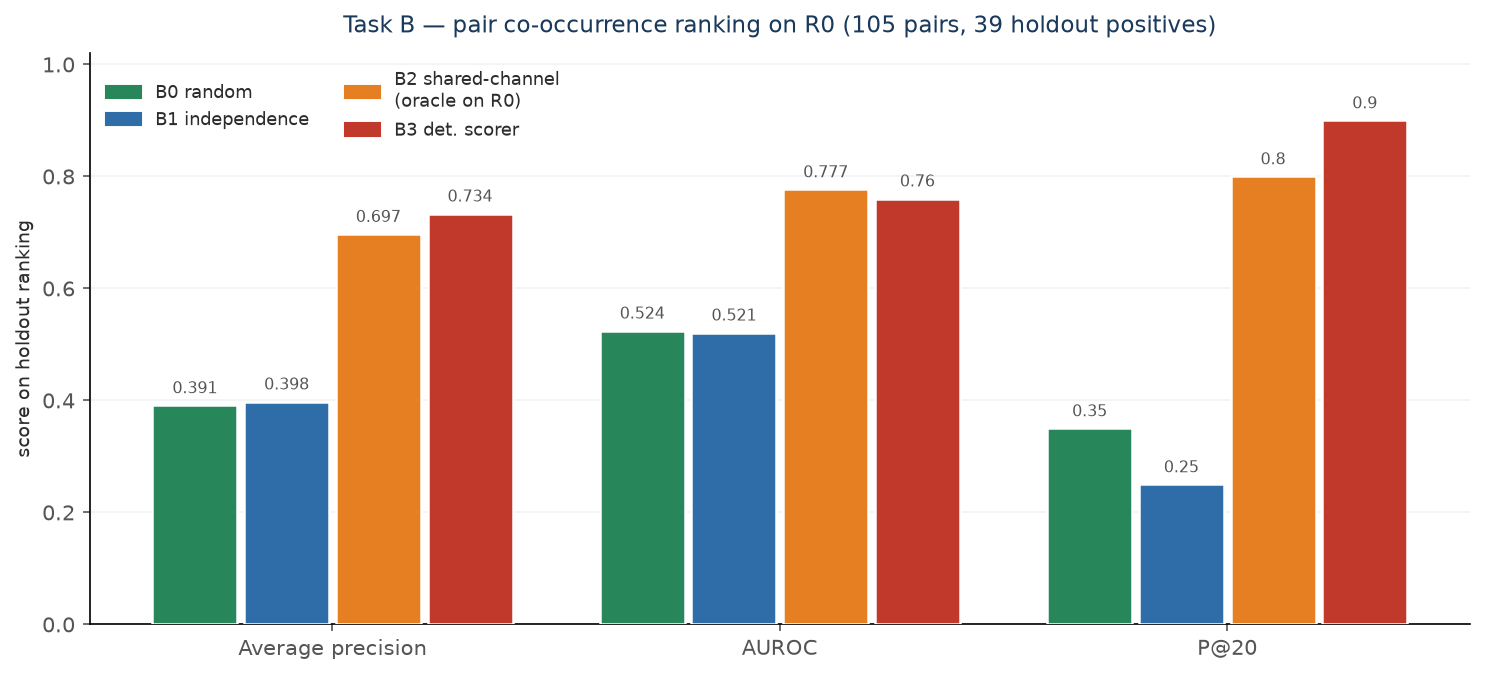
\includegraphics[width=0.98\linewidth]{figure1_taskb_baselines.png}
\caption{Task B on R0, from the shipped evaluation artifact. B2's channel
tags are the planted ground truth --- an oracle, not a deployable baseline
--- and the generator's shock-dominated marginals force B1 to near-chance,
so the honest margin is B3 over B2 on the top-weighted metrics (AP, P@20),
with B3 losing on AUROC.}
\label{fig:taskb}
\end{figure}

Pre-registered pass: AP lift over B1 $\ge$ 15\% relative. Observed lift:
\textbf{84.3\%} $\to$ \textbf{PASS}. Three things the pass does \emph{not}
mean, stated here so a validator does not have to discover them:

\begin{enumerate}[leftmargin=1.6em]
\item \textbf{The B1 bar was structurally near-unloseable on R0.} The
  generator's marginal firing is shock-dominated with near-homogeneous atom
  parameters (base quarterly rates 0.004--0.012 against channel-shock
  additions of 0.55--0.75), so the product of marginals carries almost no
  ranking signal --- B1 scores AP 0.398 against a random 0.391 --- while
  the same planted channel shocks \emph{create} the holdout labels. The
  84\% figure is therefore a function of the generator's parameters at
  least as much as of the scorer. It verifies the machinery; it is not a
  finding about the world.
\item \textbf{B2 is an oracle on this regime, not a deployable baseline.}
  Its channel tags are the planted ground truth --- the answer key. The
  honest data-only margin the table supports is \textbf{B3 over B2: +5.2\%
  AP (0.7335 vs 0.6971) and P@20 0.90 vs 0.80, while B3 loses on AUROC
  (0.761 vs 0.777)}. The metric disagreement is informative, not
  embarrassing: AP and P@20 concentrate on the top of the ranking --- the
  operative loss function for a product that surfaces a top-20 --- while
  AUROC integrates over the full ranking, where the shrinkage layer gives
  back some discrimination. Both facts are reported; preferring the
  top-weighted metrics is a product-shape argument, made explicitly rather
  than by omission.
\item \textbf{No metric carries a confidence interval.} Single frozen
  split, 105 pairs, 39 positives; the B3$-$B2 AP gap is 0.036. Bootstrap
  CIs over pairs, multi-seed regeneration of R0, and a
  $\kappa \in \{1, 4, 16\}$ sensitivity are all cheap, deterministic, and
  scheduled (proposal \S A6); until they run, the gap should be read as
  ``consistently positive on the top-weighted metrics, magnitude
  unresolved.''
\end{enumerate}

Two provenance disclosures. \emph{Hyperparameter circularity:}
\texttt{eb\_strength} $= 4$ was selected using the Task A calibration
harness \textbf{on R0}, and the GO is measured on the same single-seed R0;
$\kappa = 4$ is a bare code default with no recorded selection procedure.
One mitigating fact, found during this revision's reproduction: the shipped
Phase-1 report predates the config fields added by hardening (including
\texttt{eb\_strength}), and re-running today reproduces \textbf{every
reported metric exactly} under the enlarged config --- i.e., the Task B
result is invariant to the \texttt{eb\_strength} introduction on this
dataset, so the circularity, while real in principle, was immaterial here.
\emph{The missing baseline:} the table cannot isolate the shrinkage layer's
marginal value over ``channel knowledge plus any tie-break''; a composite
baseline (graded channel weight $\times$ empirical count) is specified and
scheduled (proposal \S A6).

\subsection{Task C --- planted structure recovery, audited}
\label{sec:taskc}

With the planted channel graph hidden, ranking pairs by train-window
co-occurrence lift recovers it: precision@30 $=$ \textbf{0.767} (23 of 30
planted edges; pre-registered threshold 0.70) $\to$ \textbf{PASS}. Four
disclosures that v1 owed the reader:

\begin{enumerate}[leftmargin=1.6em]
\item \textbf{Attribution.} Recovery is performed by a harness utility
  ranking observed co-occurrence lift --- not by the scorer's shrunk-joint
  layer. v1's abstract attributed it to ``the dependence-aware scorer'';
  this one does not.
\item \textbf{The second pre-registered metric was unpassable as written.}
  The plan requires ``planted high-risk pairs rank in top decile of U'' ---
  but 30 planted pairs cannot rank inside an 11-slot top decile
  ($\lceil 105/10 \rceil = 11$), so recall against the planted set caps at
  0.37, and ``high-risk'' is defined nowhere. The harness implements a
  different quantity --- the planted fraction \emph{of} the top decile ---
  and that is what the reported \textbf{0.909} (10/11, threshold 0.70)
  measures. The number is real; the criterion is a post-hoc
  reinterpretation of an unpassable pre-registration, and this paper now
  says so rather than presenting it as the original.
\item \textbf{Base rates.} Random selection of 30 from 105 pairs yields
  expected precision 0.286; random selection among the 54 pairs with
  \emph{any} train co-occurrence yields 0.481. Against those floors, 0.767
  is a real effect of moderate size --- not the dramatic figure it reads as
  bare.
\item \textbf{The lift normalization is inert here, and the cut is
  tie-dominated.} Ranking by raw co-occurrence \emph{count} under the same
  lexicographic tie-break reproduces precision 0.767 exactly --- and under
  other tie-break conventions count-ranking spans roughly 0.63--0.80,
  sometimes beating the lift ranking, because only 21 pairs have two or
  more co-occurrences: nine of the thirty slots go to count-1 pairs chosen
  from 33 candidates by tie-break alone. Either way the conclusion stands:
  on this regime Task C certifies that planted structure produces countable
  co-occurrence, not that the lift normalization adds value. The lift
  ranking's own top-30 cut likewise falls inside a five-way tie (ranks
  30--34 share lift 4.0) resolved by count and then id lexicography over
  ids that embed the planted channel names; that resolution moves at most
  one planted pair across the cut, and the pass margin (23 vs 21) does not
  depend on it --- but a pre-registered test should not owe any margin to
  tie-break lexicography, and a score-jittered re-run is scheduled.
\end{enumerate}

One structural note spanning \S\ref{sec:taskb}--\ref{sec:taskc}: Task B's
B3, Task C's precision, and the top-decile fraction are three views of the
same underlying train co-occurrence statistic. v1 presented them as
independent confirmations; they are one confirmation viewed three ways.

\subsection{Task A --- atom frequency calibration (an honest FAIL, now fully honest)}
\label{sec:taska}

The same harness grades the marginals. On R0 the strict rule \textbf{FAILs},
in all three of its views --- v1 quoted two and omitted the third
(Figure~\ref{fig:pit}):

\begin{itemize}[leftmargin=1.4em]
\item NLL: the model (76.34) loses to the pooled naive rate (72.47);
\item 90\% interval coverage: 0.967, above the $[0.80, 0.95]$ band;
\item \textbf{Brier (the harness's own sparse-regime fallback comparison):
  the model also loses, 0.18634 vs 0.18542} --- omitted in v1;
\item and the PIT histogram over-masses its top decile (0.233 vs 0.10
  nominal) --- the coverage pathology in distributional form, also omitted
  in v1.
\end{itemize}

The report states the two causes plainly: discrete intervals over-cover at
low rates (a regime property --- the band is unreachable), and no per-atom
model beats pooling when true rates are near-homogeneous. Two fixes
followed, both now in the algorithm: empirical-Bayes shrinkage of atom rates
toward the pool (\S\ref{sec:frequency}), and an R0$'$ count regime with a
Poisson/NB family choice.

\begin{figure}[h!]
\centering
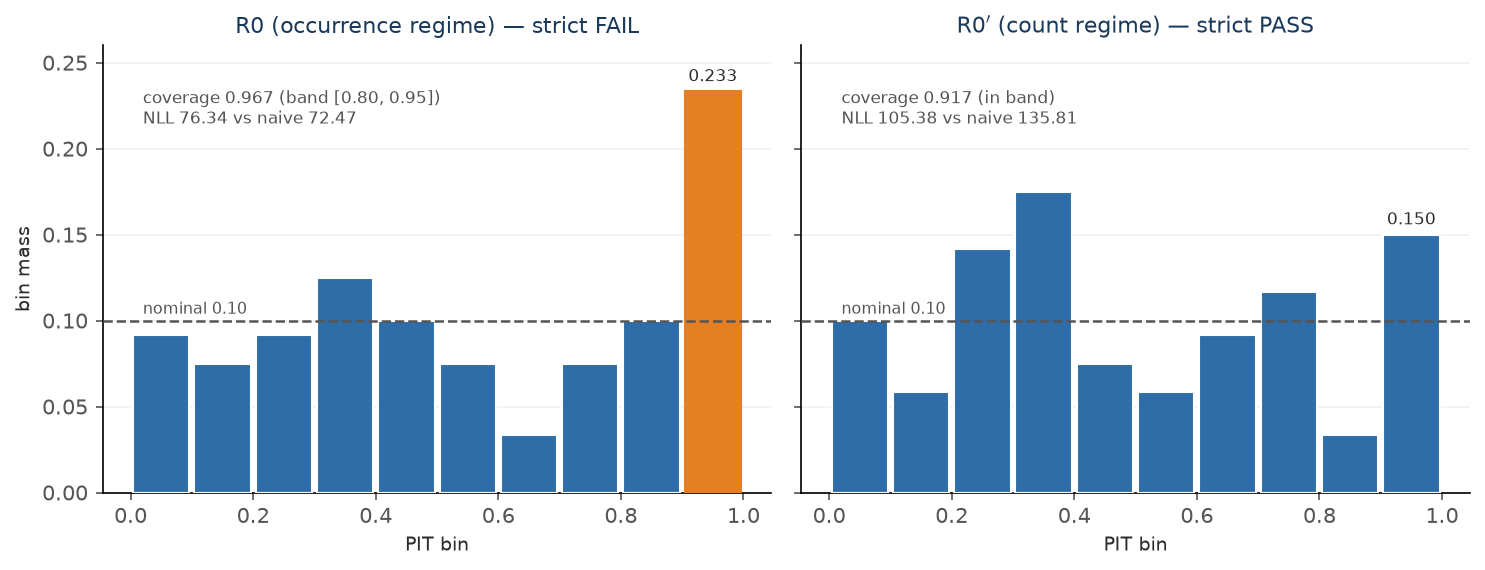
\includegraphics[width=0.98\linewidth]{figure2_pit_calibration.png}
\caption{Task A probability-integral-transform histograms from the two
calibration artifacts. Left: R0, strict FAIL --- the top-decile bin holds
0.233 of the mass (nominal 0.10), the distributional form of the interval
over-coverage. Right: the R0$'$ count regime generated for this revision,
strict PASS on all views (the labeled top-decile bin, 0.15, is not
flagged).}
\label{fig:pit}
\end{figure}

\textbf{Correction of v1's false sentence.} v1 claimed NLL then ``beats the
naive baseline on both regimes.'' It does not, and the artifact behind v1
said so. The corrected record, now backed by an on-disk artifact generated
for this revision (the R0$'$ calibration run had no stored artifact when v1
shipped --- its one favorable calibration claim was the one with no stored
evidence):

\begin{itemize}[leftmargin=1.4em]
\item \textbf{R0 (occurrence regime): strict FAIL.} NLL 76.34 vs 72.47 ---
  the pooled naive rate still wins, consistent with near-homogeneous true
  rates; pooling is simply the right model there.
\item \textbf{R0$'$ (count regime): strict PASS, on all views.} NLL 105.38
  vs 135.81; Brier 0.1708 vs 0.1766; coverage 0.917 inside the band; the
  moment-matched family choice selects negative binomial for all 15
  overdispersed cells; the PIT top-decile mass is 0.15. (This is
  \emph{stronger} than v1's hedge ``coverage still documented as
  over-covering'' --- on the generated artifact R0$'$ coverage is in band.)
\end{itemize}

The FAIL is quoted because the white paper's claim is not ``the algorithm is
right'' but ``the algorithm's failures are measured and priced in'' --- a
claim that survives only if the failures are quoted completely.

\subsection{Ablations --- reframed to what they actually show}
\label{sec:ablations}

\begin{table}[h!]
\centering\small
\begin{tabular}{@{}p{0.17\linewidth}p{0.24\linewidth}p{0.50\linewidth}@{}}
\toprule
Ablation & v1's framing & What it actually shows \\
\midrule
A1 remove dependence & ``cleanest possible confirmation the layer is the
product'' & \textbf{A wiring check.} With
\texttt{dependence\_mode="independence"} the scorer computes literally B1's
formula, so the collapse (AP 0.734 $\to$ 0.398, $=$ B1 to three decimals) is
a code identity that cannot fail; its AP drop is Task B's B3$-$B1 gap
counted a second time. Valuable as a smoke test; not design evidence. The
value evidence is \S\ref{sec:taskb}'s B3-over-B2 margin, with its caveats. \\
\addlinespace
A3 remove EVT overlay & ``tail quantiles less stable across seeds;
consistent'' & \textbf{A weak stability claim, honestly bounded.} q99
seed-CV 0.045 $\to$ 0.034 with EVT, over 3 seeds $\times \le 5$ pairs, under
a rule that fails only if EVT makes stability $>$5\% (relative)
\emph{worse} --- and the with-EVT arm substitutes the empirical q99 whenever
the overlay reports unstable. A3 shows the overlay does not hurt and
modestly helps stability. It says nothing about tail accuracy (no loss-side
task exists --- \S\ref{sec:notmeasured}). \\
\bottomrule
\end{tabular}
\end{table}

A5 (external features) stays gated: the FDR-disciplined feature registry
exists, but accepted \texttt{associational\_feature}s require human/policy
acceptance before they may act as modifiers, so the ablation activates with
the modifier path.

\subsection{External-context discipline}
\label{sec:ext}

Because time-aligning ``what else was happening'' with sparse losses is a
machine for just-so stories, external features face a gauntlet before they
may influence a rating: pre-registration of feature families, a fixed
quarterly calendar, train-only association tests with block-bootstrap CIs, a
one-shot holdout direction check, Benjamini--Hochberg FDR at $q = 0.10$,
minimum support of 8 quarters, and an \textbf{adversarial null pass} that
must write the best \emph{non-causal} explanation. Survivors are labeled
\texttt{associational\_feature} --- modifier candidates, never causal
evidence.

On the planted demo series the gauntlet's stages each did their job --- by
\emph{different} mechanisms v1 conflated: the strong planted feature was
accepted (rate ratios 14.4 and 12.0, $q < 0.1$); one noise feature
(\texttt{sanctions-regime-active}) reached the FDR stage and was rejected;
the other (\texttt{rate-hike-quarter}) --- and the weak planted feature ---
were blocked by the minimum-support gate and never reached FDR at all. Net
claim (no noise accepted) holds; the mechanism is now stated correctly.

\subsection{What the harness does not measure}
\label{sec:notmeasured}

The most important evaluation facts are the missing instruments, so they get
their own section.

\begin{itemize}[leftmargin=1.4em]
\item \textbf{No compound-level calibration task exists.} Tasks A/B/C
  calibrate atom marginals, rank pairs, and recover structure;
  \textbf{nothing anywhere tests the level of $\hat p(S)$ or its interval
  coverage.} This blind spot is load-bearing: within a zero-support stratum
  the \S\ref{sec:defects} prior defect is a constant multiplicative
  markdown, invisible to every ranking metric by construction --- the
  estimator's level bias sits precisely where the evaluation has no
  instrument. On R0 the generative truth $q_S$ is computable for every
  pair, so the instrument is cheap: interval coverage over the 105 pairs
  plus level bias stratified by expected co-occurrence under independence
  \emph{and} by (rare $\times$ supported). Scheduled, proposal \S A6; the
  mixture challenger of \S\ref{sec:defects} promotes only if it wins on
  this task.
\item \textbf{Half the output vector has no evaluation at all.} $L \mid S$
  is reported as four quantiles and a mean; no task anywhere scores loss
  quantiles against anything (A3 measures seed-\emph{stability}, not
  accuracy). The truth pack stores every atom's generative severity
  parameters, so a severity-calibration task is cheap and scheduled
  (proposal \S A6). Until it runs: \textbf{occurrence is evaluated;
  severity is reported unvalidated} --- and on the production regime the
  persisted loss numbers are additionally unit-polluted placeholders
  (\S\ref{sec:candidates}).
\item \textbf{No metric uncertainty} (\S\ref{sec:taskb}): single frozen
  split, no bootstrap, no multi-seed replication, no $\kappa$ sensitivity.
  Scheduled, proposal \S A6.
\item \textbf{Task D (expert resolution) has never run.} The only
  judgment-adjacent evidence is a properly-labeled \emph{simulated}-panel
  FAIL, which does not count in either direction; the ``workshop material''
  framing of \S\ref{sec:classes} therefore rests on an untested instrument.
\end{itemize}

\subsection{The GO decision, restated with its actual scope}
\label{sec:go}

The harness's combined recommendation on R0 is \textbf{GO}, and this
revision does not retract it --- it scopes it. GO licenses: continued
research-tier operation behind the \S\ref{sec:confidentiality} boundary, the
challenger and instrument work of the companion proposal, and workshop use
of scored realizations under the \S\ref{sec:rated} language discipline. GO
does \textbf{not} assert: a pass under the evaluation plan's stricter
Phase-1 mapping (it fails there --- \S\ref{sec:conflict}); calibrated
$\hat p$ levels (no instrument --- \S\ref{sec:notmeasured}, with a known
level defect sitting in the blind spot --- \S\ref{sec:defects}); validated
severity (\S\ref{sec:notmeasured}); or any production dependence signal
(none exists --- \S\ref{sec:conflict}). (The Phase 2 multiverse search loop
passed its own pre-registered batch-vs-loop test and was removed from
mainline on 2026-08-01: at live-data scale batch scoring does everything
production needs. The rating algorithm is unaffected --- batch is the
production path.)

% =======================================================================
\section{Limitations, stated before the conclusion}
\label{sec:limitations}

\subsection{Regime limits}
\label{sec:regimes}

\begin{itemize}[leftmargin=1.4em]
\item \textbf{R0 is synthetic.} Passing on planted structure proves the
  machinery recovers structure, not that the world has that structure ---
  and \S\ref{sec:taskb} shows the headline lift is partly a generator
  property. On the public regime (R1) Task B itself \textbf{FAILs} --- 78
  scored pairs, 4 holdout positives, lift 0.0 --- and because no pair
  co-occurs in the R1 training window, \textbf{B3 $\equiv$ B1 there:
  production scores currently carry zero empirical dependence support}
  (\S\ref{sec:conflict}). That is exactly why R0 is the decision regime and
  why the production join gates on data sufficiency rather than scoring
  anyway. Absolute calibration is not established beyond the shipped
  synthetic and sparse public-demo regimes.
\item \textbf{Compounds are rare by definition}, so holdout positives are
  few and metrics are noisy; the harness counters with proxy tasks and
  synthetic injection, not with bigger claims --- and, since v1, with the
  explicit \S\ref{sec:notmeasured} list of instruments it still lacks.
\end{itemize}

\subsection{Known defects in the shipped estimator (found in review)}
\label{sec:defects}

\begin{itemize}[leftmargin=1.4em]
\item \textbf{The dependence prior cannot hold its center for rare pairs.}
  The prior's strength is denominated in quarters ($\kappa = 4$), not
  expected co-events, so every zero-support pair receives the same constant
  markdown $\kappa/(T+\kappa) \approx 0.11$ on its independence product
  (Figure~\ref{fig:markdown}). For common pairs that markdown is evidence
  (at $q_i = 0.30$, independence expected $\approx 2.9$ co-fires in 32
  quarters; observing zero is informative). For rare pairs it is a prior
  artifact (at $q_i = 0.05$, independence predicts zero co-fires with
  probability 0.92; observing zero proves nothing) --- the technical cause
  being that with $\alpha = \kappa\, q_{\mathrm{ind}} \ll 1$ the Beta prior
  is L-shaped and ``centred on independence'' in mean only. Consequence,
  plainly: \textbf{rare, severe, never-yet-co-observed combinations --- the
  product's stated reason to exist --- are priced roughly nine times below
  the independence baseline that \S\ref{sec:problem} already calls too
  low.} Task B cannot see it (constant factors within a stratum preserve
  rankings) and no level-calibration task exists
  (\S\ref{sec:notmeasured}): the defect sits exactly in the evaluation's
  blind spot, which is why both fixes ship together --- the spike-and-slab
  mixture challenger that treats zeros as uninformative for rare pairs
  while keeping the markdown where zeros are informative (proposal \S A1;
  the spec's \S4.3 common-factor model subsumes it when data allows,
  \S A2), promoted only if it wins on the new \S\ref{sec:notmeasured}
  calibration task.
\item \textbf{In 15 of the 105 shipped audit blobs, $\hat p$ lies outside
  its own 90\% interval} --- worst row $3.1\times10^{-4}$ against
  $[0, 4.7\times10^{-11}]$, nearly seven orders of magnitude apart
  (Figure~\ref{fig:intervals}). Mechanisms in \S\ref{sec:dependence}. A
  further defect in the same construction: the interval conditions on the
  marginal point estimates $q_i$ as if known, so it understates total
  uncertainty most for thin-history atoms. Fixes scheduled (proposal
  \S A3): clip each draw, report the posterior median alongside the mean,
  flag violating rows, two-level sampling so marginal uncertainty
  propagates; the \S A1 reparameterization removes the $\alpha \ll 1$
  regime at the root. Until then a validator opening the audit blobs meets
  a point outside its interval in 14\% of rows --- the blob is honest about
  it, and now so is the paper.
\item \textbf{Atom calibration remains the weak layer} on the occurrence
  regime (\S\ref{sec:taska}): compound \emph{ranking} is the product claim;
  absolute $\hat p(S)$ values are research quantities with calibration
  tracking, not validated probabilities.
\end{itemize}

\begin{figure}[h!]
\centering
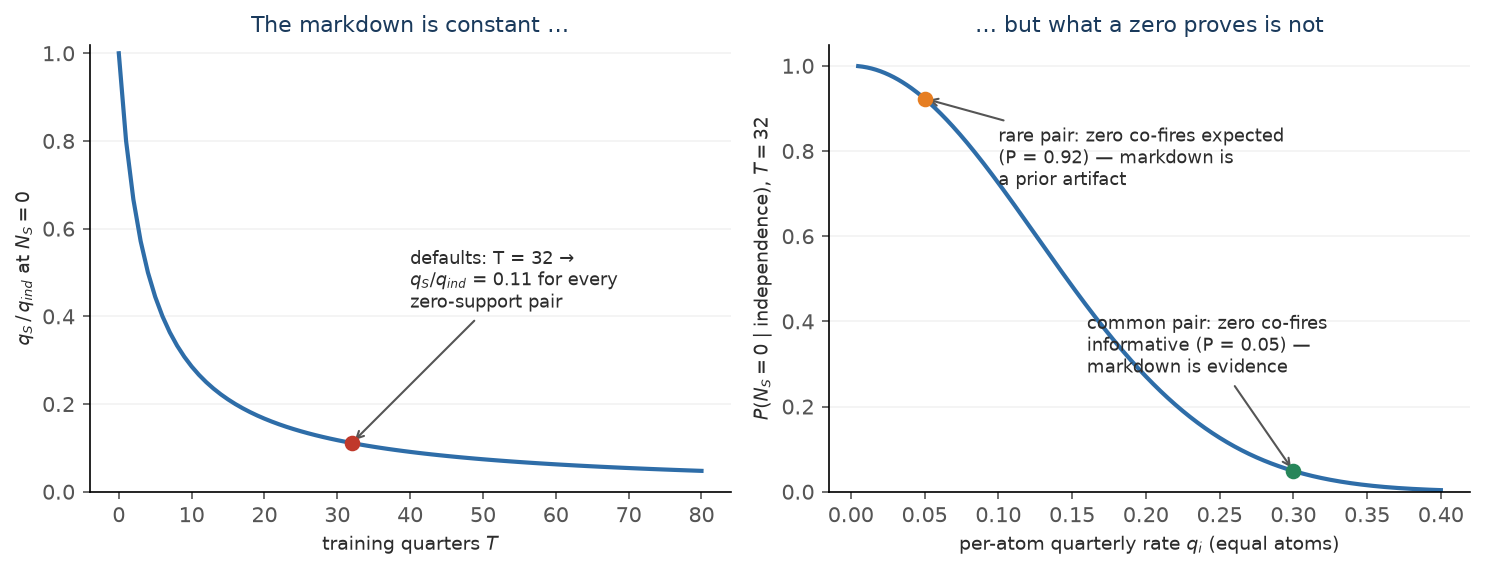
\includegraphics[width=0.98\linewidth]{figure3_rare_pair_markdown.png}
\caption{The rare-pair prior defect (formula-derived, deterministic). Left:
with no observed co-occurrence the estimator applies a constant markdown
$\kappa/(T+\kappa)$ to the independence product --- $\times 0.11$ at the
defaults. Right: what a zero observation actually proves varies enormously
--- for rare pairs, zero co-fires is the expected outcome under
independence, so the markdown is a prior artifact rather than evidence.}
\label{fig:markdown}
\end{figure}

\begin{figure}[h!]
\centering
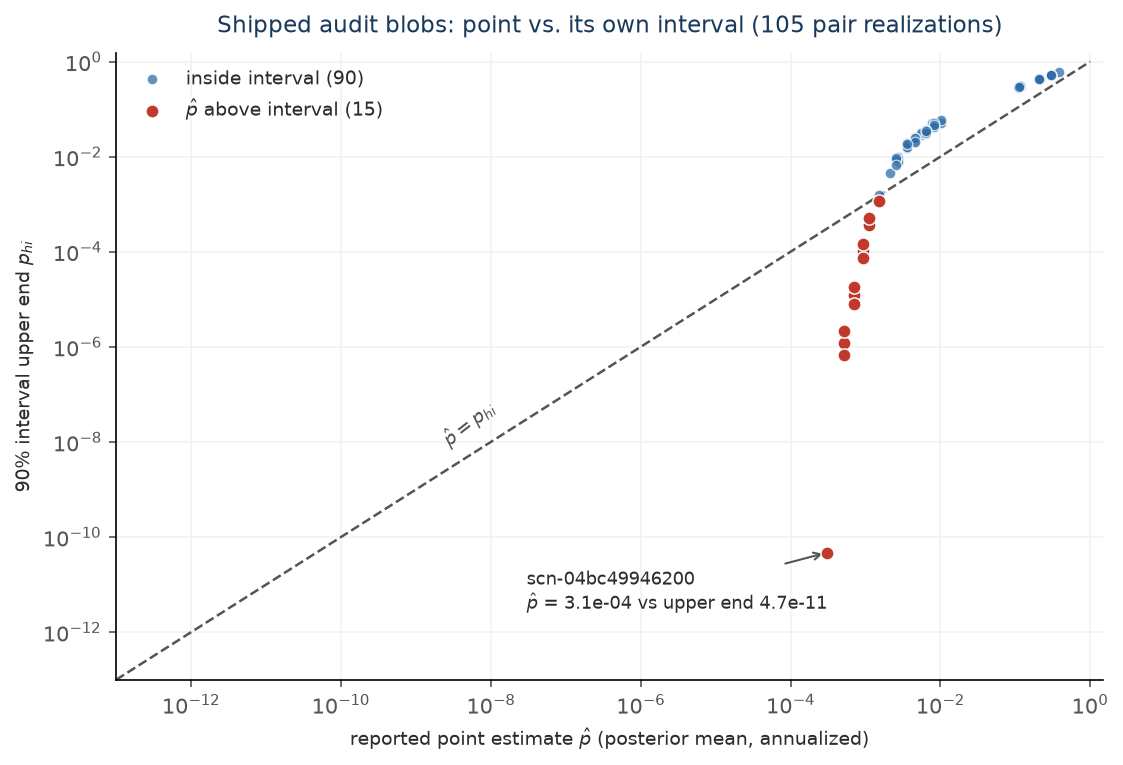
\includegraphics[width=0.88\linewidth]{figure4_interval_violations.png}
\caption{Every shipped pair realization's reported point estimate against
its own 90\% interval upper end (log--log). In 15 of 105 rows the point
lies above the interval --- in the worst row by nearly seven orders of
magnitude. Mechanisms and scheduled fixes in \S\ref{sec:dependence} and
\S\ref{sec:defects}.}
\label{fig:intervals}
\end{figure}

\subsection{Structural blind spots}
\label{sec:blindspots}

\begin{itemize}[leftmargin=1.4em]
\item \textbf{Only same-quarter co-occurrence is visible.} The occurrence
  definition, the estimator, and the labels all use the same single-quarter
  window, so a lagged cascade --- control failure in Q1 causing third-party
  failure in Q2 --- contributes nothing to the support, the labels, or the
  score. Realistic transmission narratives (\S\ref{sec:rated} stores them)
  are mostly lagged. Scheduled sensitivity: windowed co-firing
  ($w \in \{1, 2\}$ quarters), documented like the $k$-of-$n$ sensitivity;
  a Hawkes-style cross-excitation model is the higher rung (proposal
  \S A4).
\item \textbf{Emerging risks are where this engine is weakest --- by
  construction.} Three choices compound: EB shrinkage pulls a short-history
  atom toward the pooled \emph{historical} rate (for a genuinely novel
  risk, the wrong reference class); a new atom has no co-occurrence
  support, so \S\ref{sec:defects}'s below-independence markdown applies to
  its every pair; and its severity source is \texttt{pooled\_prior}. Net:
  the newer the risk, the more its score is an artifact of priors chosen
  for statistical convenience rather than relevance --- and this product's
  charter is \emph{emerging} risks. The deterministic engine has no
  mechanism to price a novel compound above its absent history. This is the
  honest limit of the data path, not a bug; v1's omission of it was the
  bug. It is the single strongest argument for activating the judgment
  channel (layers 6--7) the architecture already reserves (proposal Part B,
  esp.\ \S P3).
\item \textbf{Atom identity is string-fragile, and identity error
  masquerades as dependence.} Risk identity is exact/slugified string
  matching end to end; two records naming the same underlying risk
  differently become two atoms, and any shared evidence then registers as
  co-occurrence --- manufacturing the exact quantity this product sells.
  Semantic identity hygiene with human-gated merge is proposal work
  (\S P8).
\item \textbf{The dependence estimator is pairwise-empirical.} With sparse
  data it is a shrunk co-occurrence rate, not a causal claim; copulas and
  expert DAGs are specified higher rungs and are not yet fit. For
  $k \ge 3$ the estimator uses only the $k$-way count and the full
  independence product --- the better-supported pairwise joints are
  computed but unused (\S\ref{sec:aggregation}).
\end{itemize}

\subsection{Aggregation simplifications (roadmap tier)}
\label{sec:aggregation}

Severity dependence between atoms is not modeled (independent severities,
$\alpha_{\mathrm{overlap}} = 1.0$); event multiplicity within a quarter is
discarded where it matters most --- the loss (one severity draw per atom per
hit quarter; a compound-Poisson quarter model would use counts the pipeline
already stores); the severity blend has a discontinuity at $n = 30$ and
blends $\sigma$ linearly; the EVT overlay inherits the lognormal ceiling
(\S\ref{sec:evt}) pending data-side family selection; and $k$-way scoring
ignores pairwise information (a sharper Fr\'echet clip from pairwise joints
is the cheap fix). Tracking status, stated precisely: the count-aware MC and
$k$-way items are in the proposal (\S A5, \S A2); the severity-blend items
and data-side family selection are prescribed at spec level (algorithm-spec
\S3.2) but scheduled nowhere yet --- this list is their record.

\subsection{Contract gaps}
\S\ref{sec:gaps} is part of the limitations and is not repeated here.

% =======================================================================
\section{Conclusion}
\label{sec:conclusion}

The contribution of this work is not a new estimator --- every component is
a method model validation already trusts (\S\ref{sec:related}). It is the
\textbf{assembly discipline}: an explicit occurrence definition, shrinkage
priors centered on the skeptic's null, a tail overlay that can fail its own
stability test, an audit blob from which every digit is reconstructable, and
a pre-registered harness that has already recorded FAILs --- including
against itself --- and priced them into the design.

This revision is that discipline applied to the paper's own headlines. The
honest results are smaller than v1's and stated without protection: on a
synthetic regime whose generator makes the naive baseline near-chance, the
data path modestly out-ranks an oracle baseline on the top-weighted metrics
(+5.2\% AP, 0.90 vs 0.80 P@20) and loses to it on AUROC; structure recovery
demonstrates that planted co-occurrence is countable, against a 48\%
informed floor; atom calibration passes on the count regime and fails on the
occurrence regime; severity and score \emph{levels} are so far unvalidated
(\S\ref{sec:notmeasured}); the shipped estimator undershoots independence
for rare unobserved pairs (\S\ref{sec:defects}); and on the only real regime
the dependence layer has yet to touch a production number
(\S\ref{sec:conflict}). v1's concluding claim --- ``dependence-aware because
independence is demonstrably wrong in the tail'' --- is retired until the
level-calibration instrument exists and an estimator that holds the
skeptic's null for rare pairs ships; both are specified in the companion
proposal, with promotion gates this harness controls.

What survives unchanged is the posture: deterministic because scores must be
reproducible, humble because the falsification criteria for retiring the
algorithm are already written down --- and honest in the only way that
compounds: including where it hurts.

% =======================================================================
\clearpage
\appendix

\section{Default configuration}
\label{app:config}

\begin{center}\footnotesize
\begin{tabular}{@{}p{0.235\linewidth}lp{0.135\linewidth}p{0.40\linewidth}@{}}
\toprule
Parameter & Default & In hash & Meaning \\
\midrule
\texttt{horizon\_quarters} & 4 & yes & rating horizon (1 year) --- note \S\ref{sec:statehash}: hashed coarsened to whole years \\
\texttt{mc\_draws} & 20{,}000 & yes & Monte Carlo draws per scenario \\
\texttt{shrink\_kappa} & 4.0 & yes & dependence pseudo-count (quarters), prior centred on independence in mean (\S\ref{sec:dependence}, \S\ref{sec:defects}) \\
\texttt{n\_min} & 30 & yes & min events for a parametric severity claim \\
\texttt{pair\_support\_min} & 3 & yes & min co-firing quarters for \texttt{statistical} class \\
\texttt{marginal\_smoothing} & 0.5 & yes & add-half smoothing on occurrence (the \texttt{eb\_strength} $= 0$ fallback; missing from v1's table) \\
\texttt{eb\_strength} & 4.0 & yes & empirical-Bayes shrinkage of atom rates (pseudo-quarters) \\
\texttt{interval\_draws} & 4{,}000 & \textbf{no} (\S\ref{sec:versioning}) & Beta posterior draws for the $\hat p$ interval \\
\texttt{evt\_enabled} & true & yes & Layer 5 on/off \\
\texttt{evt\_min\_hits} & 200 & yes & min positive MC hits before the EVT overlay runs \\
\texttt{evt\_threshold\_quantile} & 0.90 & yes & POT threshold; sensitivity refits at 0.85 / 0.95 (can degrade to one-sided --- \S\ref{sec:evt}) \\
\texttt{seed} & 20260801 & no --- stored per realization & base RNG seed (per-scenario seeds derive from the state hash) \\
\texttt{dependence\_mode} & \texttt{shrunk\_empirical} & yes & \texttt{independence} activates ablation A1 \\
interval pseudo-count floor & $10^{-6}$ & \textbf{no} --- hardcoded (\S\ref{sec:versioning}) & Beta degeneracy guard \\
\bottomrule
\end{tabular}
\end{center}

\section{Reproduction}
\label{app:repro}

All evaluation figures in this paper were re-derived from fresh runs for
this revision; the commands and their expected outcomes:

\small
\begin{verbatim}
# R0 generate + Task B + Task C (writes eval_report.{json,md})
atlas-eval demo
#   expected: AP lift 0.8434 (PASS), Task C precision 0.7667 /
#   top-decile fraction 0.9091 (PASS), recommendation GO

# Task A calibration on R0 -- exits 1: the strict FAIL is expected
atlas-eval calibrate \
  --risks  generated/redesign/phase1/r0/r0_risks.json \
  --events generated/redesign/phase1/r0/r0_events.jsonl
#   expected: NLL 76.3384 vs naive 72.4738 (loses), Brier 0.1863
#   vs 0.1854 (loses), coverage 0.9667 vs [0.80, 0.95]

# R0' count regime: regenerate dataset, then calibrate -- exits 0
python -c "
import json; from pathlib import Path
from workbench_atlas.scoring.synthetic import R0Config, generate_r0
out = Path('generated/redesign/phase3/calibration-r0prime')
out.mkdir(parents=True, exist_ok=True)
ds = generate_r0(R0Config(count_model='poisson_counts'))
(out/'r0prime_risks.json').write_text(json.dumps(
    [a.to_dict() for a in ds.atoms], indent=2, sort_keys=True))
with (out/'r0prime_events.jsonl').open('w') as f:
    [f.write(json.dumps(e.to_dict(), sort_keys=True)+'\n')
     for e in ds.events]
(out/'r0prime_truth.json').write_text(json.dumps(
    ds.truth, indent=2, sort_keys=True, default=str))
"
atlas-eval calibrate \
  --risks  generated/redesign/phase3/calibration-r0prime/r0prime_risks.json \
  --events generated/redesign/phase3/calibration-r0prime/r0prime_events.jsonl \
  --out    generated/redesign/phase3/calibration-r0prime
#   expected: NLL 105.3765 vs naive 135.805 (wins), Brier 0.1708
#   vs 0.1766 (wins), coverage 0.9167 in band, NB family 15/15

atlas-eval ablations --risks ... --events ... --truth ...
python -m workbench_atlas.compound_join --force
\end{verbatim}
\normalsize

Two caveats a reproducing validator must know (both \S\ref{sec:gaps}):

\begin{enumerate}[leftmargin=1.6em]
\item \textbf{The config hash will not match the shipped artifact.} A fresh
  run reproduces every reported metric exactly but emits
  \texttt{model\_config\_hash 6219ecd3\ldots} where the shipped Phase-1
  report says \texttt{0e76a450\ldots}: the shipped report predates the
  hardening additions to the config surface (\texttt{eb\_strength},
  \texttt{dependence\_mode}, EVT fields) --- removing exactly those keys
  from today's surface reproduces the shipped hash. The metrics' invariance
  across that config change is a robustness fact (\S\ref{sec:taskb}); the
  hash mismatch is evidence-pack staleness, and re-emission is scheduled.
\item \textbf{Freshly generated reports embed stale limitation strings}
  (``EVT tail layer is a stub''; ``R1 Task B deferred'') that contradict
  \S\ref{sec:evt} and \S\ref{sec:conflict} of this paper; the strings
  predate the features. Fix scheduled with the re-emission.
\end{enumerate}

Determinism scope: identical bytes verified on the reference platform
(macOS/CPython); cross-platform bit-identity is untested
(\S\ref{sec:versioning}).

The manuscript itself rebuilds with \texttt{make all} in
\texttt{docs/research/whitepaper/} (figures regenerate from the artifacts above via
\texttt{scripts/generate\_figures.py}, then latexmk compiles this file).

\section{Evidence map: working papers, artifacts, code}
\label{app:evidence}

Every claim in this paper resolves to one of three kinds of evidence: the
pre-registered working papers that fixed the rules and the code that
produced the outcomes --- both in the repository tree, though at revision
time the \texttt{docs/redesign} $\to$ \texttt{docs/redesignv1} spec-pack
rename and the whitepaper directory are \textbf{uncommitted}, so a checkout
of HEAD predates both --- and the generated evidence artifacts, which are
never versioned: \texttt{.gitignore} excludes \texttt{generated/} entirely,
so \textbf{a fresh clone contains no evidence pack} until the
Appendix~\ref{app:repro} commands regenerate it (deterministically ---
verified again for this revision; the R0 figures reproduce exactly). v1's
claim that all three kinds were ``in this repository'' was wrong in the way
that matters to a validator's checkout. The standing options are to commit a
frozen evidence pack with hashes or to treat this appendix plus
Appendix~\ref{app:repro} as the contract: \emph{reproducible} is not
\emph{archived}, and the reader deserves the distinction stated. The R0$'$
calibration artifact cited in \S\ref{sec:taska} --- absent entirely when v1
shipped --- now exists at the path below.

\subsection{Working papers (specification pack --- \texttt{docs/research/redesignv1/})}

\begin{itemize}[leftmargin=1.4em,itemsep=1pt]
\item \texttt{algorithm-spec.md} --- normative layer stack, elicitation and
  fusion protocols, falsification
\item \texttt{evaluation-plan.md} --- pre-registered tasks A--F, baselines,
  thresholds, abandon criteria (\S\ref{sec:conflict} documents its Phase-1
  conflict with the roadmap)
\item \texttt{data-model.md} --- schemas, structural state hash, lineage
  rules (\S\ref{sec:gaps} item 2 documents the missing data coordinate)
\item \texttt{architecture.md}; \texttt{telemetry-spec.md};
  \texttt{pitch.md}; \texttt{visualization-spec.md}
\item \texttt{loop-design.md} --- candidate generation; the multiverse loop
  itself was removed from mainline on 2026-08-01
\item \texttt{risks-and-objections.md} --- the honest case against the
  system
\item \texttt{roadmap.md} --- \S1.3 is the lenient GO criterion of
  \S\ref{sec:conflict}; the decision log's ``both regimes'' NLL entry is
  corrected by \S\ref{sec:taska} and a dated correction row
\item \texttt{model-inventory.yaml} --- research-tier registration
\end{itemize}

\subsection{Primary evaluation evidence (\texttt{generated/redesign/} --- regenerable, not versioned)}

Phase 1 --- R0 go/no-go (\texttt{phase1/}):

\begin{itemize}[leftmargin=1.4em,itemsep=1pt]
\item \texttt{r0/eval\_report.md/.json} --- Task B and C results behind
  \S\ref{sec:taskb}--\ref{sec:taskc} (recommendation GO; carries the stale
  config hash and limitation strings per Appendix~\ref{app:repro})
\item \texttt{r0/r0\_risks.json}, \texttt{r0/r0\_events.jsonl},
  \texttt{r0/r0\_truth.json} --- the synthetic regime and its planted
  ground truth, including the generative severity parameters
  \S\ref{sec:notmeasured}'s scheduled loss task will score against
\item \texttt{pairs/score\_realizations.jsonl} --- one full audit blob per
  scored pair; \textbf{predates the EVT layer} (\texttt{evt: null} in all
  105 rows) and contains the 15 interval-violation rows of
  \S\ref{sec:defects} --- kept as-is until the fixes land, because the
  blobs are the evidence for the finding
\item \texttt{pairs/run\_report.json}, \texttt{pairs/telemetry.jsonl}
\end{itemize}

Phase 3 --- harness and boundary runs (\texttt{phase3/}):

\begin{itemize}[leftmargin=1.4em,itemsep=1pt]
\item \texttt{calibration/} --- Task A on R0 behind \S\ref{sec:taska}
  (strict FAIL on all three views, with cause analysis)
\item \texttt{calibration-r0prime/} --- \textbf{generated for this
  revision}: the R0$'$ dataset and its strict-PASS calibration report
\item \texttt{ablations/} --- matrix behind \S\ref{sec:ablations}
\item \texttt{r1/} --- public-regime Task B: FAIL on sparse data;
  B3 $\equiv$ B1 (\S\ref{sec:conflict})
\item \texttt{synthetic-cell-demo/} --- fictional scoring-cell exercise.
  Task B and C pass. The \texttt{aggregation\_\allowbreak report.json}
  records 65/68 accepted rows and suppressed sparse groups; the
  \texttt{egress\_\allowbreak audit.jsonl} records admitted aggregate
  features and denied sampled local-detail event rows.
\item \texttt{ext-features/} --- the \S\ref{sec:ext} screen: strong planted
  feature accepted at RR 14.4 and 12.0, $q < 0.1$; one noise feature
  FDR-rejected, the other and the weak planted feature blocked by
  min-support
\item \texttt{workshop/} --- human-facing scenario packs
\end{itemize}

\subsection{Implementation and tests}

\begin{itemize}[leftmargin=1.4em,itemsep=1pt]
\item \texttt{workbench\_atlas/scoring/scorer.py} --- Layers 1--4; module
  docstring carries the stale EVT line noted in \S\ref{sec:evt}
\item \texttt{scoring/evt.py} --- Layer 5 (GPD overlay with
  threshold-sensitivity falsification)
\item \texttt{scoring/calibration.py}, \texttt{evaluate.py},
  \texttt{ablations.py} --- the harness that produced the artifacts above
\item \texttt{scoring/ext\_features.py} --- the \S\ref{sec:ext} FDR screen
  (imports PyYAML, outside the score path)
\item \texttt{scoring/egress.py} --- local-to-external gateway with
  hash-chained audit log
\item \texttt{compound\_join.py}, \texttt{compound\_graduate.py} ---
  production monthly join and graduation (trimmed persistence per
  \S\ref{sec:gaps})
\item \texttt{tests/test\_scoring\_*.py} --- unit and integration coverage,
  including egress red-team tests, the runnable ablations, and the
  hardening tests that assert the R0$'$-only NLL win \S\ref{sec:taska} now
  states
\end{itemize}

\section{Boundary map: where LLMs touch the wider system}
\label{app:boundary}

The compound scorer (layers 1--5) is LLM-free --- verified, and the claim is
scoped to the scorer. A validator auditing the surrounding system will meet
model output in five places, listed here so the discovery costs nothing:

\begin{center}\small
\begin{tabular}{@{}cp{0.30\linewidth}p{0.34\linewidth}p{0.22\linewidth}@{}}
\toprule
\# & Touchpoint & Nature & Guard \\
\midrule
1 & Compound scoring (layers 1--5) & none --- deterministic & this paper \\
2 & Channel tags feeding candidate generation (\S\ref{sec:candidates}) &
keyword-derived, deterministic; but they are the \emph{only} production
candidate source while empirical edges stay off & \S\ref{sec:candidates};
coverage via \S P1 enrichment; empirical-edge activation itself
unscheduled \\
3 & Graduation gate & an LLM judge's clamped numeric score decides which
compounds enter the scenario library --- a model-authored number gating
publication, though never a score field & threshold + provenance tag;
boundary documented here \\
4 & Graduated prose & LLM-written narrative fields may contain numbers (the
rationale prompt cites dependence support); kept out of score fields by
\textbf{instruction, not mechanism} & review flag only; no mechanical check
scheduled \\
5 & Legacy urgency scores (outside compound scoring) & parsed largely from
LLM-authored text (likelihood words, dollar strings, foresight vocabulary);
graduated compounds currently receive arbitrary fallback constants there
(\S\ref{sec:candidates}) & exclusion / deterministic mapping scheduled
\S A7 \\
\bottomrule
\end{tabular}
\end{center}

Layers 6--7 (judgment/pooling) would be a sixth touchpoint; they are empty
in v0.1.0 (\S\ref{sec:judgment}) and their activation gates are the subject
of the companion proposal.

% =======================================================================
\begin{thebibliography}{99}

\bibitem{bh1995}
Benjamini, Y. \& Hochberg, Y. (1995).
\textit{Controlling the false discovery rate: a practical and powerful
approach to multiple testing}. Journal of the Royal Statistical Society,
Series B, 57(1).

\bibitem{bocker2008}
B\"ocker, K. \& Kl\"uppelberg, C. (2008).
\textit{Modelling and measuring multivariate operational risk with L\'evy
copulas}. Journal of Operational Risk, 3(2).

\bibitem{cooke1991}
Cooke, R. M. (1991).
\textit{Experts in Uncertainty: Opinion and Subjective Probability in
Science}. Oxford University Press.

\bibitem{cravino_book}
Cravino, N.
\textit{AI Agents in Cybersecurity}. Manuscript in preparation. Companion
practitioner reading on simulation-driven defense and AI-agent guardrails.

\bibitem{efron1975}
Efron, B. \& Morris, C. (1975).
\textit{Data analysis using Stein's estimator and its generalizations}.
Journal of the American Statistical Association, 70(350).

\bibitem{ekm1997}
Embrechts, P., Kl\"uppelberg, C. \& Mikosch, T. (1997).
\textit{Modelling Extremal Events for Insurance and Finance}. Springer.

\bibitem{ems2002}
Embrechts, P., McNeil, A. \& Straumann, D. (2002).
\textit{Correlation and dependence in risk management: properties and
pitfalls}. In \textit{Risk Management: Value at Risk and Beyond}, Cambridge
University Press.

\bibitem{sr117}
Federal Reserve / OCC (2011).
\textit{Supervisory Guidance on Model Risk Management} (SR 11-7 / OCC
2011-12).

\bibitem{frachot2001}
Frachot, A., Georges, P. \& Roncalli, T. (2001).
\textit{Loss Distribution Approach for operational risk}. Working paper,
Cr\'edit Lyonnais.

\bibitem{genest1986}
Genest, C. \& Zidek, J. V. (1986).
\textit{Combining probability distributions: a critique and an annotated
bibliography}. Statistical Science, 1(1).

\bibitem{george1993}
George, E. I. \& McCulloch, R. E. (1993).
\textit{Variable selection via Gibbs sampling}. Journal of the American
Statistical Association, 88(423).

\bibitem{hosking1987}
Hosking, J. R. M. \& Wallis, J. R. (1987).
\textit{Parameter and quantile estimation for the generalized Pareto
distribution}. Technometrics, 29(3).

\bibitem{mcneil2015}
McNeil, A., Frey, R. \& Embrechts, P. (2015).
\textit{Quantitative Risk Management: Concepts, Techniques and Tools}
(revised ed.). Princeton University Press.

\bibitem{mitchell1988}
Mitchell, T. J. \& Beauchamp, J. J. (1988).
\textit{Bayesian variable selection in linear regression}. Journal of the
American Statistical Association, 83(404).

\bibitem{moscadelli2004}
Moscadelli, M. (2004).
\textit{The modelling of operational risk: experience with the analysis of
the data collected by the Basel Committee}. Banca d'Italia, Temi di
discussione 517.

\bibitem{neslehova2006}
Ne\v{s}lehov\'a, J., Embrechts, P. \& Chavez-Demoulin, V. (2006).
\textit{Infinite-mean models and the LDA for operational risk}. Journal of
Operational Risk, 1(1).

\bibitem{nosek2018}
Nosek, B. A., Ebersole, C. R., DeHaven, A. C. \& Mellor, D. T. (2018).
\textit{The preregistration revolution}. Proceedings of the National
Academy of Sciences, 115(11).

\bibitem{ohagan2006}
O'Hagan, A. et al. (2006).
\textit{Uncertain Judgements: Eliciting Experts' Probabilities}. Wiley.

\end{thebibliography}

\end{document}
